% Chapter 2

\chapter{Funzioni esponenziali e logaritmiche } % Chapter title

\label{ch:esponenziali-logaritmi} % For referencing the chapter elsewhere, use \autoref{ch:introduction} 

%----------------------------------------------------------------------------------------
\section{Potenze}
Fissato un esponente $a \in \R$ la funzione potenza è:
\[f(x)=x^a\]
la cui definizione e dominio dipendono dal valore dell’esponente a.
\begin{itemize}
\item $a=n \in \N$
\[f(x)=x^n= \underbrace{x \times \dots \times x}_{\textbf{n volte}} \qquad \dom f=\R \qquad \im f= 
\begin{cases}
		\R \qquad \text{se n dispari} \\
		[0,+\infty )  \qquad \text{se n pari } n \neq 0 \\
		\{0\}  \qquad n = 1
\end{cases}\]

\item $a=-n\in \Z , n\in \N ,n \geq 1$
\[f(x)=x^{-n}=\frac{1}{x^n} \qquad \dom f = \R \backslash \{0\} \qquad \im f=
\begin{cases}
		\R \backslash \{0\} \qquad \text{n dispari} \\
		(0,+\infty )  \qquad \text{n pari }
\end{cases}
\]
\item $a=\frac{1}{n} \in \Z , n\in \N ,n \geq 2$
\[f(x)=x^{\frac{1}{n}}=\sqrt[n]{x} \qquad 
\dom f = 
\begin{cases}
		\R \qquad \text{n dispari} \\
		[0,+\infty )  \qquad \text{n pari }
\end{cases}
\qquad \im f=
\begin{cases}
		\R \qquad \text{n dispari} \\
		[0,+\infty) \qquad \text{n pari }
\end{cases}
\]

\item $a=\frac{m}{n} \in \Q , n\in \N ,n \geq 1 , m \in \Z$
\[f(x)=x^{\frac{m}{n}}=\sqrt[n]{m} \qquad 
\dom f = (0,+\infty)
\qquad \im f=(0,+\infty)\]

\item $a \in \R$
\[f(x)=x^a=
\begin{cases}
	\text{sup}\{x^q | q \in \Q , q \leq a\} \quad x \geq 1 \\
	\text{inf} \{x^q | q\in \Q , q \leq a\} \quad 0 < x < 1
\end{cases}
\qquad
\dom f = (0, + \infty)
\qquad
\im f = (0, + \infty)
\]


\end{itemize}


Osserviamo che:
\begin{itemize}
	\item $f(0)=0$
	\item $f(1)=1$
	\item se $n$ pari $f$ è pari
	\item se $n$ dispari $f$ è dispari
\end{itemize}

\subsection{Proprietà delle potenze}
\begin{itemize}
\item $x^{n+m}=x^n x^m$
\item $(x^n)^m=x^{nm}$
\end{itemize}

\paragraph{Osservazioni}
\[f(x)=x^0=1 \quad \forall x \in \R\]
\[0^0=1\]

\subsubsection{Dimostrazioni}

\[x^{n+m}= \underbrace{x \times \dots \times x}_{\text{n+m volte}}=\underbrace{(x \times \dots \times x)}_{\text{n volte}}\times \underbrace{x \times \dots \times x}_{\text{m volte}}=x^{n+m}\]

\[(x^{n})^m= \underbrace{x^n \times \dots \times x^n}_{\text{m volte}}\]

\[x^n=x^{n+0}=x^n x^0 \qquad x\neq 0\]
\[x^0 = 1 \quad \forall x \in \R\]

\begin{figure}[H]
{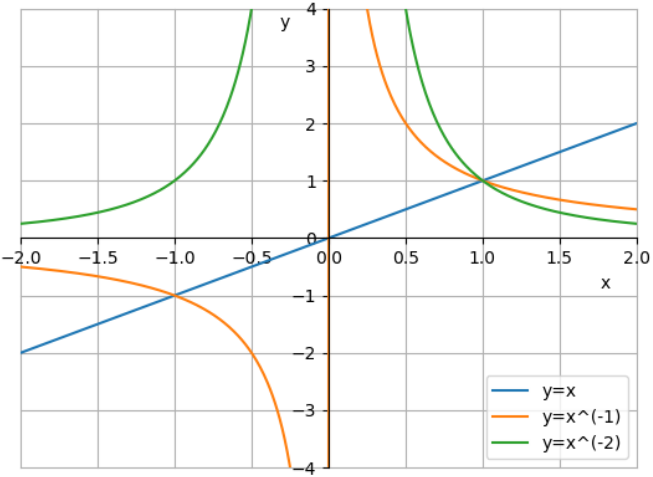
\includegraphics[width=.9\linewidth]{gfx/3/potenze.png}}
\caption{Grafici di funzioni di potenze.}\label{fig:potenze}
\end{figure}

\section{Esponenziale}
Fissata la base $a>0$ con $a \neq 1$, la funzione esponenziale è
\[f(x)=a^x \qquad \dom f = \R \qquad \im f = (0,+\infty)\]
Se si sceglie come base il numero di Nepero $e=2.71828\dots > 1$, la funzione esponenziale si denota:
\[f(x)=e^x=\exp x\]

\subsection{Proprietà}
\begin{enumerate}
	\item se $a>1$, allora la funzzione $a^x$ è strettamente crescente
	\item se $0<a<1$, allora la funzione $a^x$ è strettamente decrescente
	\item se $0<a<b$ con $a,b \neq 1$
	\[\begin{cases}
		a^x<b^x \qquad x>0 \\
		a^x > b^x \qquad x<0
	\end{cases}\]
	\item valgono le seguenti proprietà:
	\begin{itemize}
	\item $a^0=1$
	\item $a^1=a$
	\item $a^{x_1+x_2}=a^{x_1+x_2} \qquad x_1,x_2 \in \R$
	\item $a^{-x}=(\frac{1}{a})^x \qquad x \in \R$
	\item $(a^x)^b = a^{bx} \qquad x,b \in \R$
	\end{itemize}
\end{enumerate}

\begin{figure}[H]
{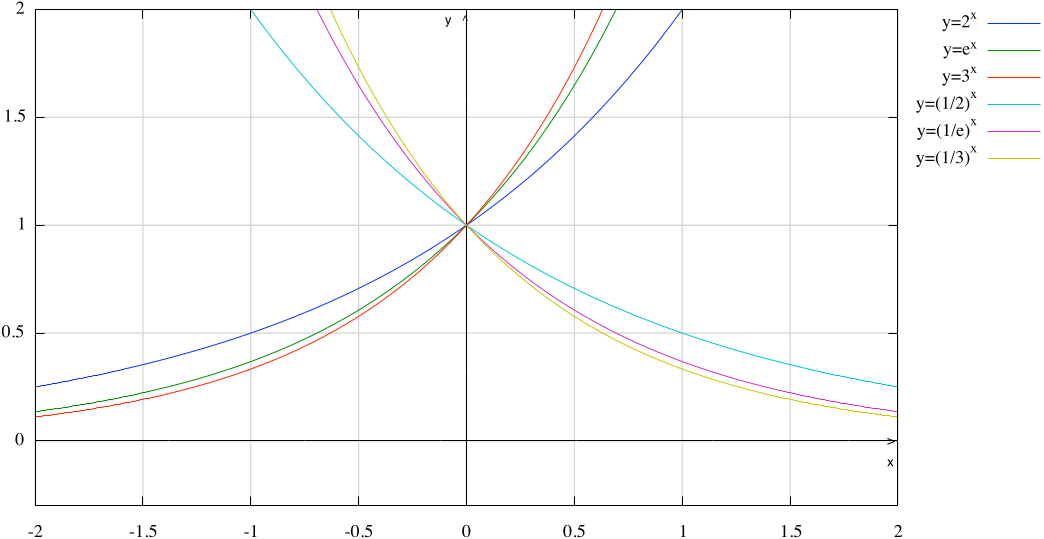
\includegraphics[width=.9\linewidth]{gfx/3/esponenziali.png}}
\caption{Grafici di funzioni esponenziali.}\label{fig:esponenziali}
\end{figure}

\section{Logaritmo}
Fissata la base $a>0$ con $a\neq 1$, la funzione logaritmo
\[f(x)=\log_a x \qquad \dom f = (0,+\infty) \qquad \im f = \R\]
è definita come la funzione inversa della funzione esponenziale $a^x$. Se si sceglie come base il numero di Nepero \textit{e}, il logaritmo si denota:
\[f(x)=\log_e = \log x = \ln x\]

\begin{enumerate}
	\item se $a>1$, allora la funzione $\log_a x$ è strettamente crescente
	\item se $0<a<1$, allora la funzione $\log_a x$ è strettamente decrescente
	\item se $0<a<b$ con $a,b\neq 1$
	\[\begin{cases}
	\log_a x > \log_b x \qquad se x>1 \\
	\log_a x < \log_b x \qquad se 0<x<1 \\
	\end{cases}\]
	\item valgono le seguenti proprietà:
	\begin{itemize}
		\item $\log_a a^x = x \qquad x>1$
		\item $a^{\log_a x}=x \qquad x>0$
		\item $\log_a 1 = 0$
		\item $\log_a a = 1$
		\item $\log_a (x_1 x_2)= \log_a x_1 + \log_a x_2 \qquad x_1,x_2 > 0$
		\item $\log_a (\frac{x_1}{x_2})=\log_a x_1 - \log_a x_2 \qquad x_1,x_2 > 0$
		\item $\log_a x^b = b \log_a x \qquad x>0, b \in \R$
		\item $\log_a x= \frac{\log_b x}{\log_b a}=\frac{\ln x}{\ln a}\qquad x>0,b>0,b\neq 1$
		\item $a^x = e^{(\ln a)x} \qquad x\in \R, a>0, a \neq 1$
	\end{itemize}
\end{enumerate}

\begin{figure}[H]
{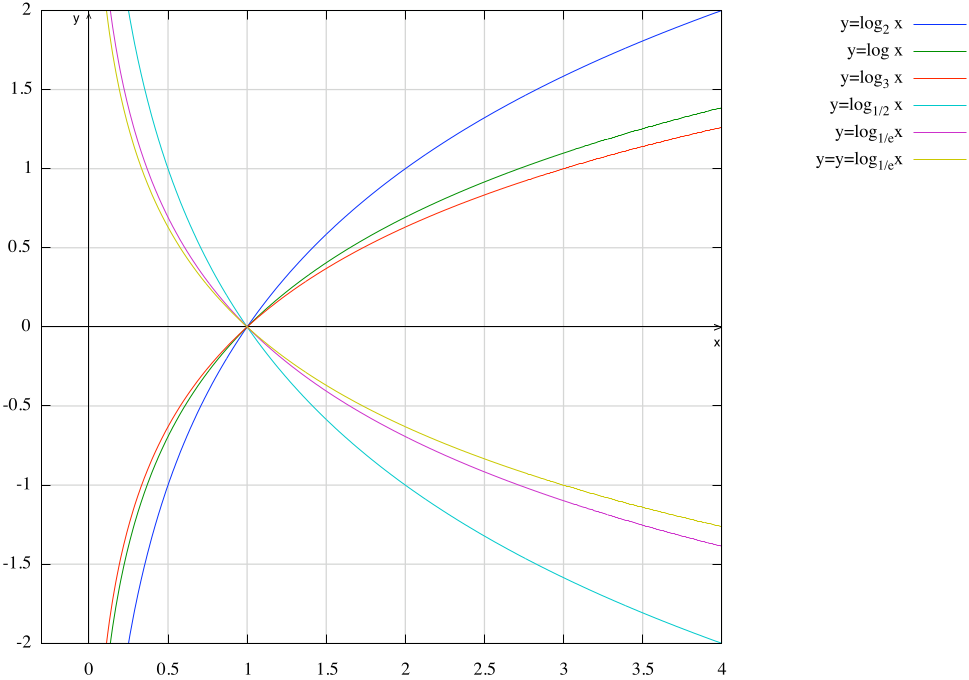
\includegraphics[width=.9\linewidth]{gfx/3/logaritmi.png}}
\caption{Grafici di funzioni logaritmiche.}\label{fig:logaritmi}
\end{figure}